% ৪.x HTML Document-এর মৌলিক কাঠামো
\section{HTML Document-এর মৌলিক কাঠামো}

\begin{learningbox}
এই টপিক শেষে শিক্ষার্থী পারবে:
\begin{itemize}
\item HTML document structure কী তা ব্যাখ্যা করতে।
\item \texttt{<!DOCTYPE html>}, \texttt{<html>}, \texttt{<head>}, \texttt{<title>} ও \texttt{<body>} tag-এর কাজ লিখতে।
\item \texttt{<head>} ও \texttt{<body>} অংশের পার্থক্য বুঝতে।
\item একটি basic HTML file লিখে \texttt{.html} extension দিয়ে save করতে।
\item HSC practical ও board exam-এর জন্য standard HTML structure মনে রাখতে।
\end{itemize}
\end{learningbox}

\subsection{ভূমিকা}

HTML tag, element ও attribute জানা থাকলে একটি সম্পূর্ণ web page-এর গঠন বোঝা সহজ হয়। HTML file-এর code এলোমেলোভাবে লেখা যায় না; browser যেন document-এর শুরু, page title, metadata এবং visible content ঠিকভাবে বুঝতে পারে, সে জন্য একটি নির্দিষ্ট structure অনুসরণ করা হয়।

HSC ICT-তে basic HTML program লেখার সময় সাধারণত \texttt{<html>}, \texttt{<head>}, \texttt{<title>} এবং \texttt{<body>} অংশ ব্যবহার করে web page তৈরি দেখানো হয়। আধুনিক HTML-এ এর শুরুতে \texttt{<!DOCTYPE html>} এবং বাংলা text ঠিকভাবে দেখানোর জন্য \texttt{<meta charset="UTF-8">} ব্যবহার করা ভালো।


\begin{definitionbox}{HTML Document Structure}
HTML Document Structure হলো একটি HTML web page-এর মৌলিক গঠন, যেখানে কোন tag কোথায় থাকবে এবং browser কোন অংশ কীভাবে বুঝবে তা নির্ধারিত থাকে।
\end{definitionbox}

\subsection{Basic HTML Structure}

\begin{examplebox}{Code}
\begin{verbatim}
<!DOCTYPE html>
<html>
<head>
  <meta charset="UTF-8">
  <title>My First Web Page</title>
</head>
<body>
  <h1>Welcome to HSC ICT</h1>
  <p>This is my first HTML web page.</p>
</body>
</html>
\end{verbatim}
\end{examplebox}

\begin{examplebox}{Output ধারণা}
Browser tab-এ \texttt{My First Web Page} দেখা যাবে। Web page-এর body area-তে \texttt{Welcome to HSC ICT} heading এবং নিচে paragraph text দেখা যাবে।
\end{examplebox}

\begin{keypointbox}{আধুনিক practice note}
\begin{itemize}
\item \texttt{<html>} tag-এ \texttt{lang} attribute দিলে page-এর ভাষা বোঝা সহজ হয়।
\item \texttt{<meta charset="UTF-8">} বাংলা ও অন্যান্য Unicode text ঠিকভাবে দেখাতে সাহায্য করে।
\item \texttt{<meta name="viewport" content="width=device-width, initial-scale=1.0">} mobile-friendly display-এর জন্য কাজে লাগে।
\item \texttt{<head>} অংশে title, metadata, CSS link ও script link রাখা হয়।
\end{itemize}
\end{keypointbox}

\subsection{Structure-এর প্রধান অংশ}

\subsubsection{\texttt{<!DOCTYPE html>}}

\begin{definitionbox}{Document type declaration}
\texttt{<!DOCTYPE html>} হলো document type declaration, যা browser-কে জানায় যে document-টি modern HTML বা HTML5 standard অনুসরণ করে লেখা হয়েছে।
\end{definitionbox}

\begin{itemize}
\item এটি HTML tag নয়, declaration।
\item সাধারণত HTML document-এর একদম শুরুতে লেখা হয়।
\item Browser-কে standard mode-এ page render করতে সাহায্য করে।
\item HSC basic code-এ অনেক সময় না দেখালেও modern HTML code-এ এটি লেখা ভালো।
\end{itemize}

\subsubsection{\texttt{<html>} tag}

\begin{definitionbox}{Root element}
\texttt{<html>} tag হলো HTML document-এর root element; এর ভিতরে সম্পূর্ণ web page-এর code লেখা হয়।
\end{definitionbox}

\begin{examplebox}{Code}
\begin{verbatim}
<html>
  ...
</html>
\end{verbatim}
\end{examplebox}

\begin{itemize}
\item \texttt{<html>} tag document-এর শুরু নির্দেশ করে।
\item \texttt{</html>} tag document-এর শেষ নির্দেশ করে।
\item এর ভিতরে সাধারণত দুইটি প্রধান অংশ থাকে: \texttt{<head>} এবং \texttt{<body>}।
\end{itemize}

\subsubsection{\texttt{<head>} tag}

\begin{definitionbox}{Head section}
\texttt{<head>} tag হলো HTML document-এর এমন অংশ যেখানে page সম্পর্কিত তথ্য, title, style, script, link এবং meta information রাখা হয়।
\end{definitionbox}

\begin{examplebox}{Code}
\begin{verbatim}
<head>
  <title>Page Title</title>
</head>
\end{verbatim}
\end{examplebox}

\begin{itemize}
\item এই অংশের content সাধারণত browser window-এর main page area-তে সরাসরি দেখা যায় না।
\item Page title, character encoding, CSS link, script link ইত্যাদি এখানে লেখা যায়।
\item HSC exam-এ \texttt{<head>} অংশের কাজ হিসেবে page-related information উল্লেখ করতে হবে।
\end{itemize}

\begin{keypointbox}{Head-এর ভিতরে থাকতে পারে}
\begin{itemize}
\item \texttt{<title>}
\item \texttt{<meta>}
\item \texttt{<link>}
\item \texttt{<style>}
\item \texttt{<script>}
\item \texttt{<base>}
\end{itemize}
\end{keypointbox}

\subsubsection{\texttt{<meta charset="UTF-8">}}

\begin{definitionbox}{Character encoding}
\texttt{<meta charset="UTF-8">} হলো metadata tag, যা document-এর character encoding নির্ধারণ করে।
\end{definitionbox}

\begin{examplebox}{Code}
\begin{verbatim}
<meta charset="UTF-8">
\end{verbatim}
\end{examplebox}

\begin{itemize}
\item বাংলা, ইংরেজি এবং অধিকাংশ ভাষার character ঠিকভাবে দেখাতে সাহায্য করে।
\item এটি \texttt{<head>} tag-এর ভিতরে লেখা হয়।
\item বাংলা content যুক্ত web page-এ এটি ব্যবহার করা ভালো অভ্যাস।
\end{itemize}

\subsubsection{\texttt{<title>} tag}

\begin{definitionbox}{Page title}
\texttt{<title>} tag browser tab বা title bar-এ web page-এর title প্রদর্শন করে।
\end{definitionbox}

\begin{examplebox}{Code}
\begin{verbatim}
<title>My First Web Page</title>
\end{verbatim}
\end{examplebox}

\begin{itemize}
\item এটি \texttt{<head>} tag-এর ভিতরে লেখা হয়।
\item এটি page body-এর ভিতরে দেখা যায় না।
\item Bookmark বা search result-এ page title বোঝাতে সাহায্য করে।
\end{itemize}

\begin{center}
\begin{tabular}{|p{0.24\textwidth}|p{0.58\textwidth}|}
\hline
\textbf{Tag} & \textbf{কোথায় দেখা যায়} \\
\hline
\texttt{<title>} & Browser tab/title bar-এ \\
\hline
\texttt{<h1>} & Web page-এর visible body area-তে \\
\hline
\end{tabular}
\end{center}

\subsubsection{\texttt{<body>} tag}

\begin{definitionbox}{Visible content section}
\texttt{<body>} tag হলো HTML document-এর প্রধান অংশ, যেখানে web page-এর দৃশ্যমান content লেখা হয়।
\end{definitionbox}

\begin{examplebox}{Code}
\begin{verbatim}
<body>
  <h1>Welcome</h1>
  <p>This is a paragraph.</p>
</body>
\end{verbatim}
\end{examplebox}

\begin{itemize}
\item Web page-এ যে text, image, link, table, list বা form দেখা যায়, তা \texttt{<body>} অংশে লেখা হয়।
\item \texttt{<body>} tag-এর বাইরে visible heading বা paragraph লেখা উচিত নয়।
\item HSC practical code-এ body অংশ সবচেয়ে বেশি ব্যবহৃত হয়।
\end{itemize}

\begin{keypointbox}{Body-এর ভিতরে থাকতে পারে}
\begin{itemize}
\item Heading: \texttt{<h1>} থেকে \texttt{<h6>}
\item Paragraph: \texttt{<p>}
\item Image: \texttt{<img>}
\item Hyperlink: \texttt{<a>}
\item List: \texttt{<ul>}, \texttt{<ol>}, \texttt{<li>}
\item Table: \texttt{<table>}
\item Form: \texttt{<form>}
\end{itemize}
\end{keypointbox}

\subsection{Head ও Body-এর পার্থক্য}

\begin{center}
\begin{tabular}{|p{0.22\textwidth}|p{0.32\textwidth}|p{0.32\textwidth}|}
\hline
\textbf{বিষয়} & \textbf{\texttt{<head>}} & \textbf{\texttt{<body>}} \\
\hline
কাজ & Page সম্পর্কিত তথ্য রাখে & Page-এর visible content রাখে \\
\hline
Browser-এ সরাসরি দেখা যায়? & সাধারণত না & হ্যাঁ \\
\hline
Example tag & \texttt{<title>}, \texttt{<meta>}, \texttt{<style>} & \texttt{<h1>}, \texttt{<p>}, \texttt{<img>}, \texttt{<a>} \\
\hline
ব্যবহার & metadata, title, CSS, script link & heading, paragraph, image, table, form \\
\hline
HSC focus & setting, style, script, title & browser-এ যা দেখা যায় \\
\hline
\end{tabular}
\end{center}

\subsection{HTML Structure Diagram}

\begin{center}
\fbox{\parbox{0.88\textwidth}{
\centering
\textbf{HTML Document}\\[4pt]
\texttt{<!DOCTYPE html>}\\
$\downarrow$\\
\texttt{<html>}\\
$\swarrow \hspace{2cm} \searrow$\\
\texttt{<head>} \hspace{2cm} \texttt{<body>}\\
\texttt{title, meta, style} \hspace{1.1cm} \texttt{heading, paragraph, image, link}
}}
\end{center}

\begin{center}
\textbf{HTML Document Tree}\\[6pt]
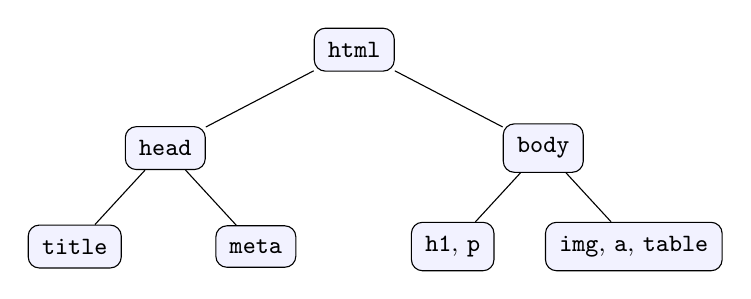
\begin{tikzpicture}[
  level distance=1.25cm,
  level 1/.style={sibling distance=4.8cm},
  level 2/.style={sibling distance=2.3cm},
  every node/.style={draw, rounded corners, align=center, fill=blue!5, inner sep=5pt, font=\small}
]
\node {\texttt{html}}
  child { node {\texttt{head}}
    child { node {\texttt{title}} }
    child { node {\texttt{meta}} }
  }
  child { node {\texttt{body}}
    child { node {\texttt{h1}, \texttt{p}} }
    child { node {\texttt{img}, \texttt{a}, \texttt{table}} }
  };
\end{tikzpicture}
\end{center}

\begin{keypointbox}{Tree থেকে code বোঝার নিয়ম}
Tree diagram-এ parent tag-এর ভিতরে child tag থাকে। যেমন \texttt{<html>} tag-এর ভিতরে \texttt{<head>} ও \texttt{<body>} থাকে। আবার \texttt{<body>} tag-এর ভিতরে visible content যেমন heading, paragraph, image, link, list ও table লেখা হয়।
\end{keypointbox}

\begin{examplebox}{Code}
\begin{verbatim}
<!DOCTYPE html>
<html>
  <head>
    <title>Page Title</title>
  </head>

  <body>
    Visible content
  </body>
</html>
\end{verbatim}
\end{examplebox}

\subsection{Complete Example: College Web Page}

\begin{examplebox}{Code}
\begin{verbatim}
<!DOCTYPE html>
<html>
<head>
  <meta charset="UTF-8">
  <title>ABC College</title>
</head>
<body>
  <h1>ABC College</h1>
  <p>Welcome to our college website.</p>
  <p>Here you can find notice, result and admission information.</p>
</body>
</html>
\end{verbatim}
\end{examplebox}

\begin{center}
\begin{tabular}{|p{0.30\textwidth}|p{0.54\textwidth}|}
\hline
\textbf{Code} & \textbf{কাজ} \\
\hline
\texttt{<!DOCTYPE html>} & HTML5 document ঘোষণা করে \\
\hline
\texttt{<html>} & সম্পূর্ণ document ধরে \\
\hline
\texttt{<head>} & page সম্পর্কিত তথ্য রাখে \\
\hline
\texttt{<meta charset="UTF-8">} & character encoding নির্ধারণ করে \\
\hline
\texttt{<title>} & browser tab title দেখায় \\
\hline
\texttt{<body>} & visible content রাখে \\
\hline
\texttt{<h1>} & বড় heading দেখায় \\
\hline
\texttt{<p>} & paragraph দেখায় \\
\hline
\end{tabular}
\end{center}

\subsection{HTML File Save করার নিয়ম}

HTML code লেখার পর file save করতে হবে \texttt{.html} বা \texttt{.htm} extension দিয়ে।

\begin{examplebox}{File name example}
\texttt{index.html}, \texttt{home.html}, \texttt{about.html}
\end{examplebox}

\begin{enumerate}
\item Notepad বা VS Code open করো।
\item HTML code লিখো।
\item File save করো \texttt{index.html} নামে।
\item File browser দিয়ে open করো।
\item Output browser-এ দেখো।
\end{enumerate}

\begin{mistakebox}{সাধারণ ভুল}
\begin{itemize}
\item \texttt{<!DOCTYPE html>} না লেখা।
\item \texttt{<head>} tag-এর ভিতরে visible content লেখা।
\item \texttt{<body>} tag-এর বাইরে heading বা paragraph লেখা।
\item \texttt{<title>} tag-কে page heading মনে করা।
\item closing tag না দেওয়া।
\item file \texttt{.txt} হিসেবে save করা।
\item বাংলা text ঠিকভাবে দেখানোর জন্য \texttt{UTF-8} না দেওয়া।
\item \texttt{<head>} ও \texttt{<body>} tag-এর order ভুল করা।
\end{itemize}
\end{mistakebox}

\begin{boardbox}{সঠিক order মনে রাখো}
\texttt{DOCTYPE} $\rightarrow$ \texttt{html} $\rightarrow$ \texttt{head} $\rightarrow$ \texttt{title/meta} $\rightarrow$ \texttt{body} $\rightarrow$ visible content
\end{boardbox}

\subsection{পরীক্ষার জন্য সংক্ষিপ্ত উত্তর}

HTML document একটি নির্দিষ্ট কাঠামো অনুসরণ করে লেখা হয়। আধুনিক HTML document-এর শুরুতে \texttt{<!DOCTYPE html>} লেখা হয়। এরপর \texttt{<html>} tag-এর মধ্যে সম্পূর্ণ document থাকে। \texttt{<head>} অংশে web page সম্পর্কিত তথ্য, title, metadata, style ও script রাখা হয়। \texttt{<title>} tag browser tab-এ page title প্রদর্শন করে। \texttt{<body>} অংশে web page-এর দৃশ্যমান content যেমন heading, paragraph, image, hyperlink, list, table ও form লেখা হয়।

\subsection{ছোট প্রশ্নোত্তর}

\begin{enumerate}
\item HTML document-এর root element কোনটি?\\
\textbf{উত্তর:} \texttt{<html>}।

\item HTML document-এর visible content কোন tag-এর ভিতরে লেখা হয়?\\
\textbf{উত্তর:} \texttt{<body>} tag-এর ভিতরে।

\item Web page-এর title browser tab-এ দেখাতে কোন tag ব্যবহৃত হয়?\\
\textbf{উত্তর:} \texttt{<title>} tag।

\item \texttt{<head>} tag-এর কাজ কী?\\
\textbf{উত্তর:} Page সম্পর্কিত তথ্য, title, metadata, style ও script রাখার জন্য \texttt{<head>} tag ব্যবহৃত হয়।

\item \texttt{<!DOCTYPE html>} কেন ব্যবহার করা হয়?\\
\textbf{উত্তর:} Browser-কে জানাতে যে document-টি modern HTML বা HTML5 standard অনুসরণ করে লেখা হয়েছে।

\item বাংলা text ঠিকভাবে দেখাতে কোন meta tag ব্যবহার করা ভালো?\\
\textbf{উত্তর:} \texttt{<meta charset="UTF-8">}।
\end{enumerate}

\subsection{Exam Focus MCQ}

\begin{enumerate}
\item HTML document-এর root element কোনটি?\\
ক) \texttt{<head>} \quad খ) \texttt{<title>} \quad গ) \texttt{<html>} \quad ঘ) \texttt{<body>}

\item Browser tab-এ page title দেখাতে কোন tag ব্যবহৃত হয়?\\
ক) \texttt{<h1>} \quad খ) \texttt{<title>} \quad গ) \texttt{<body>} \quad ঘ) \texttt{<p>}

\item Web page-এর visible content কোন element-এর ভিতরে থাকে?\\
ক) \texttt{<head>} \quad খ) \texttt{<body>} \quad গ) \texttt{<title>} \quad ঘ) \texttt{<meta>}

\item Page সম্পর্কিত metadata কোন অংশে থাকে?\\
ক) \texttt{<body>} \quad খ) \texttt{<head>} \quad গ) \texttt{<table>} \quad ঘ) \texttt{<img>}

\item Modern HTML document-এর শুরুতে কোন declaration লেখা হয়?\\
ক) \texttt{<html>} \quad খ) \texttt{<!DOCTYPE html>} \quad গ) \texttt{<body>} \quad ঘ) \texttt{<title>}
\end{enumerate}

\begin{boardbox}{Answer key}
১-গ, ২-খ, ৩-খ, ৪-খ, ৫-খ
\end{boardbox}
